% TODO:
% - 

%%%%%%%%%%%%%%%%%%%%%%%%%%%%%%%%%%%%%%%%%%%%%%%%%%%%
% documentclss
%\documentclass[]{beamer}
%\documentclass[handout]{beamer} %Drucker Version
\documentclass[draft]{beamer}


%%%%%%%%%%%%%%%%%%%%%%%%%%%%%%%%%%%%%%%%%%%%%%%%%%%%
% packages

\usepackage[utf8]{inputenc}
\usepackage[ngerman]{babel}
\usepackage[T1]{fontenc}

\usepackage{setspace}
\usepackage{ellipsis}
\usepackage{microtype}
\usepackage{lmodern}

\usepackage{lscape}
\usepackage{booktabs}			% \toprule, \midrule und \bottomrule in Tabellen
\usepackage{multirow}
\usepackage{paralist}

\usepackage{scrhack} 
\usepackage{listings}
\lstset{
    language=C,
    breaklines=true,
    breakatwhitespace=true
    basicstyle=\footnotesize,
    numbers=left,
    numberstyle=\footnotesize,
    stepnumber=1,
    numbersep=5pt,
    extendedchars=true,
    inputencoding=utf8,
    breakindent=30pt,
    escapeinside={\%(}{\%)},
    captionpos=b
}

%\usepackage[pdftex]{graphicx} % Bereits von Beamer geladen
\graphicspath{{../Master_Thesis/images/}}
\usepackage{tikz}
\usepackage{wrapfig}
\usepackage{caption}         
\usepackage{subcaption}      
\usepackage{pgfgantt}        
\usepackage{rotating} 		

\hypersetup{
    pdftex,
    bookmarks, bookmarksopen, bookmarksopenlevel=1, bookmarksnumbered=true,
    pdfpagemode={UseNone},
    pdfpagelayout={SinglePage},
    plainpages=false,
    pdfkeywords={AUTOSAR, Virtualisierung, ECU, Python, CAN},
    pdfsubject={Virtualisierung von AUTOSAR Softwarekomponenten für die Erprobung},
    pdftitle={Virtualisierung von AUTOSAR Softwarekomponenten für die Erprobung},
    pdfauthor={Martin Wichmann},
}



\newcommand{\inputImage}[1]{\input{../Master_Thesis/images/#1}}
% Bild einfügen:
%\centering
%\resizebox{0.3\linewidth}{!}{\inputImage{autosar_overview.dia}}

\newtranslation[to=ngerman]{Example}{Beispiel}

\usetheme{Warsaw}

\AtBeginSection[]
{
   \begin{frame}
        \frametitle{Inhaltsübersicht}
        \tableofcontents[currentsection,hideallsubsections]
   \end{frame}
}



%%%%%%%%%%%%%%%%%%%%%%%%%%%%%%%%%%%%%%%%%%%%%%%%%%%%
% Title
\author{Martin Wichmann}
\title[Virtualisierung von AUTOSAR Softwarekomponenten]{Virtualisierung von AUTOSAR Softwarekomponenten für die Erprobung}
\subtitle{Kolloquium zur Masterarbeit}
\date{\today}
\institute{Ostfalia Hochschule für angewandte Wissenschaften}




%%%%%%%%%%%%%%%%%%%%%%%%%%%%%%%%%%%%%%%%%%%%%%%%%%%%
% begin document
\begin{document}

\begin{frame}
\maketitle
\end{frame}


\begin{frame}
\frametitle{Inhaltsübersicht}
\tableofcontents[hideallsubsections] % Einstellungen siehe Beamer User Guide Seite 99
\end{frame}





%%%%%%%%%%%%%%%%%%%%%%%%%%%%%%%%%%%%%%%%%%%%%%%%%%%%%%%%%%%%%%%%%%%5
% Einleitung
\section{Einleitung}
\label{sec:einleitung}

%%%%%
\begin{frame}
\frametitle{Einleitung}
% TODO:
% - Warum das ganze?
\end{frame}

%%%%%%%%%%
\subsection{Motivation}
% TODO:
% - Woraus entstand die Arbeit
%%%%%
\begin{frame}
\frametitle{TODO}
    \begin{figure}[ht]
        \centering
        \resizebox{\linewidth}{!}{\inputImage{gantt}}
        \caption{TODO}
        \label{fig:TODO}
    \end{figure}
\end{frame}

%%%%%%%%%%
\subsection{Zielsystem}
% TODO:
% - Was sollte bei dem Projekt rauskommen
%%%%%
\begin{frame}
\frametitle{TODO}
    \begin{figure}[ht]
        \centering
        \resizebox{\linewidth}{!}{\inputImage{arch_begin.dia}}
        \caption{TODO}
        \label{fig:TODO}
    \end{figure}
\end{frame}



%%%%%%%%%%%%%%%%%%%%%%%%%%%%%%%%%%%%%%%%%%%%%%%%%%%%%%%%%%%%%%%%%%%5
% Grundlagen
\section{Grundlagen}
\label{sec:grundlagen}

%%%%%
\begin{frame}
\frametitle{Überblick}

\end{frame}




%%%%%%%%%%
\subsection{Virtualisierung}
%%%%%
\begin{frame}
\frametitle{TODO}
    \begin{figure}
        \centering
        \begin{subfigure}[b]{0.49\textwidth}
            \centering
            \inputImage{virt_type1.dia}
            \caption{Type 1-Hypervisor}
            \label{fig:hypervisor_type1}
        \end{subfigure}
        \begin{subfigure}[b]{0.49\textwidth}
            \centering
            \inputImage{virt_type2.dia}
            \caption{Type 2-Hypervisor}
            \label{fig:hypervisor_type2}
        \end{subfigure}
        \caption{Hypervisor Kategorien}
        \label{fig:hypervisor}
    \end{figure}
\end{frame}

%%%%%
\begin{frame}
\frametitle{TODO}
    \begin{figure}[ht]
        \centering
        \inputImage{arinc653.dia}
        \caption[ARINC 653 Architektur Übersicht]{ARINC 653 Architektur Übersicht\cite{arinc653_wr}}
        \label{fig:arinc_653}
    \end{figure}
\end{frame}





%%%%%%%%%%
\subsection{AUTOSAR}
%%%%%
%\begin{frame}[plain] % TODO: vielleicht plain da das Bild groß ist
\begin{frame}
\frametitle{TODO}
    \begin{figure}[p]
        \centering
        \resizebox{\linewidth}{!}{\inputImage{autosar_overview.dia}}
        \caption{Autosar Überblick}
        \label{fig:autosar_overview}
    \end{figure}
\end{frame}

%%%%%
\begin{frame}
\frametitle{TODO}
    \begin{figure}[ht]
        \centering
        \resizebox{\linewidth}{!}{\inputImage{Autosar_Prozess.dia}}
        \caption{AUTOSAR-Entwicklungs-Prozess}
        \label{fig:autosar_prozess}
    \end{figure}
\end{frame}

%%%%%
\begin{frame}
\frametitle{TODO}
    \begin{figure}[ht]
        \centering
        \resizebox{\linewidth}{!}{\inputImage{autosar_layer.dia}}
        \caption{AUTOSAR-Schichtenmodell}
        \label{fig:autosar_layer}
    \end{figure}
\end{frame}

%%%%%
\begin{frame}
\frametitle{TODO}
    \begin{figure}[ht]
        \centering
        \resizebox{\linewidth}{!}{\inputImage{autosar_refined_layer.dia}}
        \caption{AUTOSAR-Schichtenmodell mit genauerer Aufteilung}
        \label{fig:autosar_refined_layer}
    \end{figure}
\end{frame}

%%%%%
\begin{frame}
\frametitle{TODO}
    \begin{figure}[ht]
        \centering
        \inputImage{komm_beispiel.dia}
        \caption[Struktur der AUTOSAR-Kommunikation]{Struktur der AUTOSAR-Kommunikation für das Senden und Empfangen einer CAN-Botschaft}
        \label{fig:komm_beispiel}
    \end{figure}
\end{frame}




%%%%%%%%%%
\subsection{Netzwerkmanagment}
%%%%%
\begin{frame}
\frametitle{TODO}

\end{frame}




%%%%%%%%%%
\subsection{Funktionale Sicherheit}
%%%%%
\begin{frame}
\frametitle{TODO}
    \begin{figure}[!htbp]
        \center
        \inputImage{ISO_26262_Lifecycle.dia}
        \caption[Sicherheitslebenszyklus nach ISO 26262]{Sicherheitslebenszyklus nach ISO 26262 (vgl. \cite{iso26262})}
        \label{fig:lifecycle}
    \end{figure}
\end{frame}







%%%%%%%%%%%%%%%%%%%%%%%%%%%%%%%%%%%%%%%%%%%%%%%%%%%%%%%%%%%%%%%%%%%5
% Umsetzung
\section{Umsetzung}
\label{sec:umsetzung}

%%%%%
\begin{frame}
\frametitle{Überblick}
    \begin{figure}[ht]
        \centering
        \inputImage{arch_finished.dia}
        \caption{Vollständige Architektur}
        \label{fig:arch_finished}
    \end{figure}
\end{frame}




%%%%%%%%%%
\subsection{Virtualisierung}
%%%%%
\begin{frame}
\frametitle{TODO}

\end{frame}




%%%%%%%%%%
\subsection{Kommunikation Linux und AUTOSAR}
%%%%%
\begin{frame}
\frametitle{TODO}

\end{frame}




%%%%%%%%%%
\subsection{Kommunikation AUTOSAR und Scheinwerfer-ECU}
%%%%%
\begin{frame}
\frametitle{TODO}

\end{frame}




%%%%%%%%%%
\subsection{Entwicklung AUTOSAR Komponente}
%%%%%
\begin{frame}
\frametitle{TODO}
    \begin{figure}[ht]
        \centering
        \resizebox{\linewidth}{!}{\inputImage{SMLS_Modell.dia}}
        \caption{Entwickeltes AUTOSAR Modell}
        \label{fig:smls_modell}
    \end{figure}
\end{frame}




%%%%%%%%%%
\subsection{Entwicklung steuernde Komponente}
%%%%%
\begin{frame}
\frametitle{TODO}
    \begin{figure}
        \centering
        \begin{subfigure}[b]{0.59\textwidth}
            \centering
            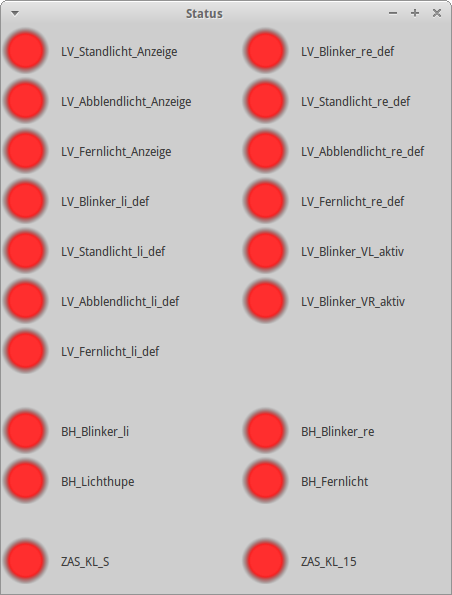
\includegraphics[width=\textwidth]{vcan_app_status}
            \caption{Status-Fenster}
            \label{fig:vcan_app_status}
        \end{subfigure}
        \begin{subfigure}[b]{0.39\textwidth}
            \centering
            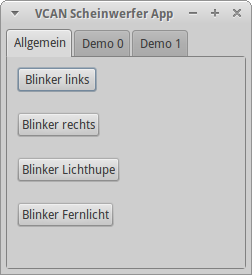
\includegraphics[width=\textwidth]{vcan_app_control}
            \caption{Kontroll-Fenster}
            \label{fig:vcan_app_control}
        \end{subfigure}
        \caption{Oberfläche der VCAN-Applikation}
        \label{fig:vcan_app}
    \end{figure}
\end{frame}





%%%%%%%%%%%%%%%%%%%%%%%%%%%%%%%%%%%%%%%%%%%%%%%%%%%%%%%%%%%%%%%%%%%5
% Fazit
\section{Analyse und Fazit}
\label{sec:analyse_fazit}

%%%%%%%%%%
\subsection{Analyse}
%%%%%
\begin{frame}
\frametitle{TODO}
    \begin{figure}
        \centering
        \begin{subfigure}[b]{0.49\textwidth}
            \centering
            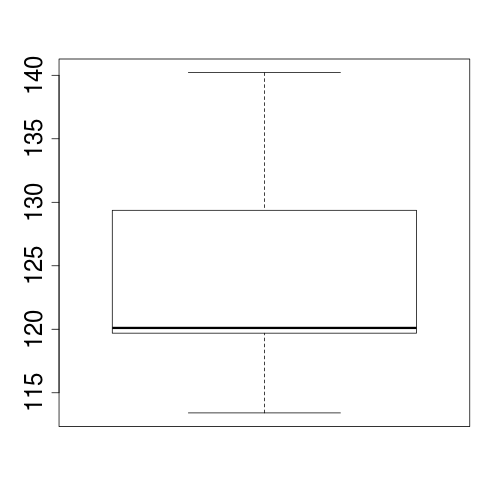
\includegraphics[width=\textwidth]{boxplot_as}
            \caption{Zeitverhalten AUTOSAR}
            \label{fig:boxplot_as}
        \end{subfigure}
        \begin{subfigure}[b]{0.49\textwidth}
            \centering
            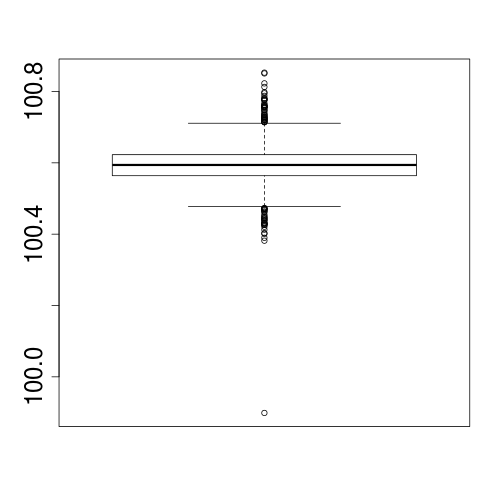
\includegraphics[width=\textwidth]{boxplot_vcan}
            \caption{Zeitverhalten VCAN-API}
            \label{fig:boxplot_vcan}
        \end{subfigure}
        \caption[Zeitanalyse des VCAN als Boxplots]{Zeitanalyse des VCAN als Boxplots (Angaben in ms)}
        \label{fig:timinganalyse}
    \end{figure}
\end{frame}



%%%%%%%%%%
\subsection{Fazit und Ausblick}
%%%%%
\begin{frame}
\frametitle{Fazit}

\end{frame}


%%%%%
\begin{frame}
\frametitle{Ausblick}

\end{frame}










%%%%%%%%%%%%%%%%%%%%%%%%%%%%%%%%%%%%%%%%%%%%%%%%%%%%%%%%%%%%%%%%%%%5
% Literaturangaben
\appendix
\section*{Literatur}
\label{sec:Literatur}

\begin{frame}


\begin{thebibliography}{10}

\bibitem[1]{1} \textsc{Olaf Kindel, Mario Driedrich}: {\em Softwareentwicklung mit AUTOSAR: Grundlagen, Engineering, Management in der Praxis.} dpunkt.verlag, 2009.

\bibitem[2]{2} \textsc{Peter Löw, Roland Pabst, Erwin Petry}: {\em Funktionale Sicherheit in der Praxis.} dpunkt.verlag, 2010.

\bibitem[3]{3} \textsc{AUTOSAR}: {\em Technical Overview.} Online unter: \url{http://autosar.org/download/R3.1/AUTOSAR_TechnicalOverview.pdf}

\bibitem[4]{4} \textsc{AUTOSAR}: {\em Layered Software Architecture.} Online unter: \url{http://autosar.org/download/R3.1/AUTOSAR_LayeredSoftwareArchitecture.pdf}

\end{thebibliography}


\end{frame}

\end{document}

